\newpage
\chapter{Prospects of Higgs pair production at Run-3 and HL-LHC}
\label{HL-LHC}

With the full Run-2 data, the 95\% CL interval for \kl modifier is -1.5 $\leq$ \kl $\leq$ 6.7 using the \HHyybb decay channel. At the end of Run-3, an expected addition of integrated luminosity of 300 \ifb, and at the end of HL-LHC, the integrated luminosity should reach 3000 \ifb at a centre-of-mass energy of 14 TeV. As the measurement of statistically limited, the Higgs pair production search will benefit from the luminosity increase and can achieve a precision of 50\% on \kl at 68\% CL at the end of HL-LHC [Ref to European strategy]. Prospects for the measurement of the trilinear Higgs self-coupling at Run-3 and HL-LHC will be presented in this chapter. 

\section{Further \HHyybb improvements}
\label{HL-LHC:Run-3}

Several improvements to the \HHyybb analysis strategy are possible in the next round. Significant enhancement can be achieved if we consider the different items presented in this thesis (not applied at Run-2 analysis):
\begin{itemize}
    \item Even with fewer variables, the DNN categorization described in Section \ref{HHyybb:ObjEvt:DNN} shows promising results. Considering this DNN at next round with the addition of the topness, HT and missing transverse energy variables, around 10\% improvement in the sensitivity of the analysis should be achievable. 
    \item Additional improvement to the \mbb resolution can be achieved with the usage of the Kinematic Fit (KF), described in Appendix \ref{Adx4}. The KF brings an additional 10\% improvement to the \mbb resolution which can be translated to 2-5\% improvement on the analysis significance. It was shown in Figures \ref{fig:Adx4:HH:0Jet} and \ref{fig:Adx4:HH:1Jet} that the fit is less constrained for high \kl values, with the current \kl interval, \kl values larger than 6 are rejected, few \% of improvement are possible considering low \kl values.
\end{itemize}

\subsection{Photon identification with CNN in \HHyybb}
\label{HL-LHC:Run-3:CNN}

Improving photon identification (PID) is critical for \HHyybb. Using the algorithm introduced in Section \ref{gamma:CNN} the PID efficiency is improved significantly. In \HHyybb channel, this improvement leads to an enhancement of the signal acceptance. The developed CNN is applied to photons from the \HHyybb simulated events.  Figure \ref{fig:HL-LHC:Run-3:CNN:E} shows the efficiency of the Tight WP for both cut-based and CNN algorithms as a function of photon energy and pseudorapidity. The CNN over-performs the cut-based and shows an efficiency closed to 100\% in the full \eT spectrum. It is another validation of the CNN in a different event topology.
\begin{figure}[htbp]
    \centering
     \subfloat[as function of \eT][as function of \eT]{\includegraphics[width=0.45\textwidth]{Ch6/Img/Eff_MixtureNN_All_Inclusive_Tight_E.pdf}}
    \subfloat[as function of $|\eta|$][as function of $|\eta|$]{\includegraphics[width=0.45\textwidth]{Ch6/Img/Eff_MixtureNN_All_Inclusive_Tight_ETA.pdf}}
    \begin{tcolorbox}[colback=black!5!white, colframe=white!75!black]
    \caption{Photon identification efficiency of cut-based Run-2 ID algorithm (blue) and the CNN ID algorithm (red) as function of photons \eT and $|\eta|$ from \HHyybb simulated events. Tight isolation is applied as baseline.}
    \label{fig:HL-LHC:Run-3:CNN:E}
    \end{tcolorbox}
\end{figure}

The \HHyybb events are characterized with two photons from H$\to\gamma\gamma$ decay with an average energy of $m_H$/2 in which the efficiency is around 99.7\% as shown in Figure \ref{fig:HL-LHC:Run-3:CNN:E}. The increase in the PID efficiency for each photon can be translated to $\sim$15\% improvement in the signal acceptance as shown in the \myy distribution in Figure \ref{fig:HL-LHC:Run-3:CNN:M}. This also true for single Higgs backgrounds.\\
 
\begin{figure}[htbp]
    \centering
    \includegraphics[width=0.5\textwidth]{Ch6/Img/Eff_MixtureNN_All_Inclusive_Tight_M.pdf}
     \begin{tcolorbox}[colback=black!5!white, colframe=white!75!black]
    \caption{\myy invariant mass distribution for two selected photon with cut-based algorithm (blue) and CNN algorithm (red).}
    \label{fig:HL-LHC:Run-3:CNN:M}
    \end{tcolorbox}
\end{figure}

For the continuum $\gamma\gamma$+jets background, the PID efficiency is shown in Figure \ref{fig:HL-LHC:Run-3:CNN:Cont:E}. The same improvement can be achieved for the continuum background. Figure \ref{fig:HL-LHC:Run-3:CNN:Cont:M} shows the \myy spectrum with an improvement of 15\% in the statistics. With the CNN algorithm, the continuum statistics can be enhanced by 15\% which will slightly improve the background modelling, thus reduce the spurious signal systematics and improve the analysis significance with approximately 7.3\%. The $b$-jet requirement in \HHyybb leads to high $\gamma\gamma$ purity as described in Section \ref{HHyybb:Modelling:Bkg}. For H$\to\gamma\gamma$ analysis, an improvement in the $\gamma\gamma$ purity is expected with the CNN algorithm.

\begin{figure}[htbp]
    \centering
    \includegraphics[width=0.5\textwidth]{Ch6/Img/Eff_Tight_All_Inclusive_Tight_E.pdf}
    \begin{tcolorbox}[colback=black!5!white, colframe=white!75!black]
    \caption{Photon identification efficiency of cut-based Run-2 ID algorithm (blue) and the CNN ID algorithm (red) as function of photons \eT from $\gamma\gamma$+jets simulated events. Tight isolation is applied as baseline.}
    \label{fig:HL-LHC:Run-3:CNN:Cont:E}
    \end{tcolorbox}
\end{figure}

\begin{figure}[htbp]
    \centering
    \includegraphics[width=0.5\textwidth]{Ch6/Img/Eff_Tight_All_Inclusive_Tight_M.pdf}
     \begin{tcolorbox}[colback=black!5!white, colframe=white!75!black]
    \caption{\myy invariant mass distribution of the continuum $\gamma\gamma$+jets for two selected photon with cut-based algorithm (blue) and CNN algorithm (red).}
    \label{fig:HL-LHC:Run-3:CNN:Cont:M}
    \end{tcolorbox}
\end{figure}

\section{Expected results from Run-2+Run-3 combination}
\label{Run-3}

Several detector upgrades are planned for the Run-3, most of those upgrades are do not have a big impact on the \HHyybb efficiency.  As mentioned before, the expected integrated luminosity at the end of Run-3 is around 300 \ifb. If we consider the same \HHyybb analysis strategy at the end of Run-3, the \HHyybb results will be almost comparable to the combination of ATLAS and CMS full Run-2 analysis presented in Section \ref{HHyybb:CMS}. Given the expected similarity in the LHC beams and data taking conditions, a combination of the Run-2 and Run-3 data is considered in the following. Combining the full Run-2 and Run-3 leads to a total integrated luminosity of 439 \ifb. \\

The estimation of \HHyybb analysis performances with the combined Run-2 and Run-3 data is performed by extrapolating the full Run-2 \HHyybb to 439 \ifb. The extrapolation is set by scaling the full Run-2 workspace to 439/139$\sim$3.2. To allow for an easy extrapolation, impacts from reconstruction algorithms are neglected. Given the assumption that \HHyybb analysis is statistically dominated, No systematic uncertainties are considered. \\

The expected upper 95\% CL limits on the Higgs pair production cross-section as a function of Higgs self-coupling \kl is shown in Figure \ref{fig:Run-3:Limit} for both full Run-2 and extrapolation to Run-2+Run-3. The expected limit for SM is found to be 2.6 times SM expectations. With the Run-2+Run-3 data the SM HH limit can be improved by a factor of 2. The expected \kl interval at 95\% CL from the limit scan is [-0.7, 6].

\begin{figure}[htbp]
    \centering
    \includegraphics[width=0.5\textwidth]{Ch6/Img/kappa_lambda_Run_2_Run_3_stat.pdf}
     \begin{tcolorbox}[colback=black!5!white, colframe=white!75!black]
    \caption{The 95\% CL expected upper limits on the HH production cross-section as function of \kl. The $\pm$1 and $\pm$2 bands are shown for the Run-2 results. The expected allowed \kl intervals are also reported.}
    \label{fig:Run-3:Limit}
    \end{tcolorbox}
\end{figure}

An Asimov dataset with the background-only hypothesis was created, and maximum likelihood fits of this dataset were performed with different \kl hypotheses. The negative logarithm of the ratio of the maximum likelihood for \kl to that for the fit with \kl= 1 is shown in Figure \ref{fig:Run-3:LH} for both Run-2 and Run-2+Run-3. The 1$\sigma$ and the 2$\sigma$ confidence interval (CI) constraints on \kl from this curve are shown in Table \ref{tab:Run-3:kl}. It can be seen in Figure \ref{fig:Run-3:LH} that there are typically two minima. The first minimum is located at \kl= 1 as the signal hypothesis used to create the Asimov dataset. The second minimum is observed at a \kl value that corresponds to a similar fitter signal yield with respect to the \kl point at the first minimum, which is a consequence of a higher cross-section, but lower acceptance and worse signal-to-background separation. The measured signal strength is 1.0 $\pm$ 1.25 considering only statistical uncertainties. The expected median significance of the SM HH signal relative to the background-only hypothesis is 0.87 $\sigma$. 

\begin{table}[htbp]
    \centering
    \begin{tabular}{ccc}
    \hline\hline 
        Scenario & 1$\sigma$ CI & 2$\sigma$ CI \\
    \hline    
        Run-2 Stat. Only & [-1.3, 6.4]  & [-2.9, 8] \\
        Run-2+Run-3 Stat. Only & [-0.4, 5.3] & [-1.5, 6.6] \\
    \hline\hline 
    \end{tabular}
    \begin{tcolorbox}[colback=black!5!white, colframe=white!75!black]
    \caption{Constraints on \kl from the likelihood ratio rest performed on the Asimov dataset created from the background and the \kl= 1 signal, as shown in Figure \ref{fig:Run-3:LH}.}
    \label{tab:Run-3:kl}
    \end{tcolorbox}
\end{table}

\begin{figure}[htbp]
    \centering
    \includegraphics[width=0.5\textwidth]{Ch6/Img/likelihood_subplot_Run3.pdf}
    \begin{tcolorbox}[colback=black!5!white, colframe=white!75!black]
    \caption{Negative natural logarithm of the ratio of the maximum likelihood for \kl to the maximum likelihood for \kl= 1. The dashed lines at 0.5 and 2.0 indicate the values corresponding to a 1$\sigma$ and 2$\sigma$ confidence interval, respectively (assuming an asymptotic $\chi^2$ distribution of the test statistic).}
    \label{fig:Run-3:LH}
    \end{tcolorbox}
\end{figure}

\section{Prospects at HL-LHC}
\label{HL-LHC:HL-LHC}

As described in Section \ref{chap2:Upgrad}, the HL-LHC is a planned upgrade of the LHC and supposed to collect an integrated luminosity of 3000 \ifb. It will be operated at $\sqrt{s} = $ 14 TeV and will start after the long shut-down three around 2027. An upgrade of the ATLAS detector and trigger system is planned which will compensate the higher pileup density which will be around 200 collisions per bunch crossing. Due to the higher pileup, photons and jets energy resolutions are expected to slightly degrade, but this might be compensated by better photon reconstruction techniques. With the ITk, the $b$-tagging efficiency will be improved by 8\% per jet, while remaining the same rejection efficiency. A prospects study of the Higgs pair production at HL-LHC is performed in the context of the European strategy in 2019. In this study, three HH decay channels are considered : \bbbb, \bbtt and \bbyy. For \bbbb and \bbtt the 36 \ifb analysis are kept unchanged and extrapolated to 3000 \ifb at 14 TeV, while a completely new truth MC-based analysis is performed for \bbyy. In the following the European strategy results for \HHyybb are presented.

\subsection{Estimation for European strategy 2019}
As mentioned above, the prospect of \HHyybb at HL-LHC are performed through the use of truth-level Monte Carlo samples generated at $\sqrt{s} = $ 14 TeV. To emulate the response of the upgraded ATLAS detector at the HL-LHC, the final state particles at truth level are smeared assuming the pileup density of 200 at HL-LHC. In contrary to 36 \ifb analysis, the projection improves the sensitivity by including a BDT categorization. The BDT is trained to separated the SM HH signal from the backgrounds. The BDT response for signal and background is shown in Figure \ref{fig:HL-LHC:36ifb:BDT}. 

\begin{figure}[htbp]
    \centering
    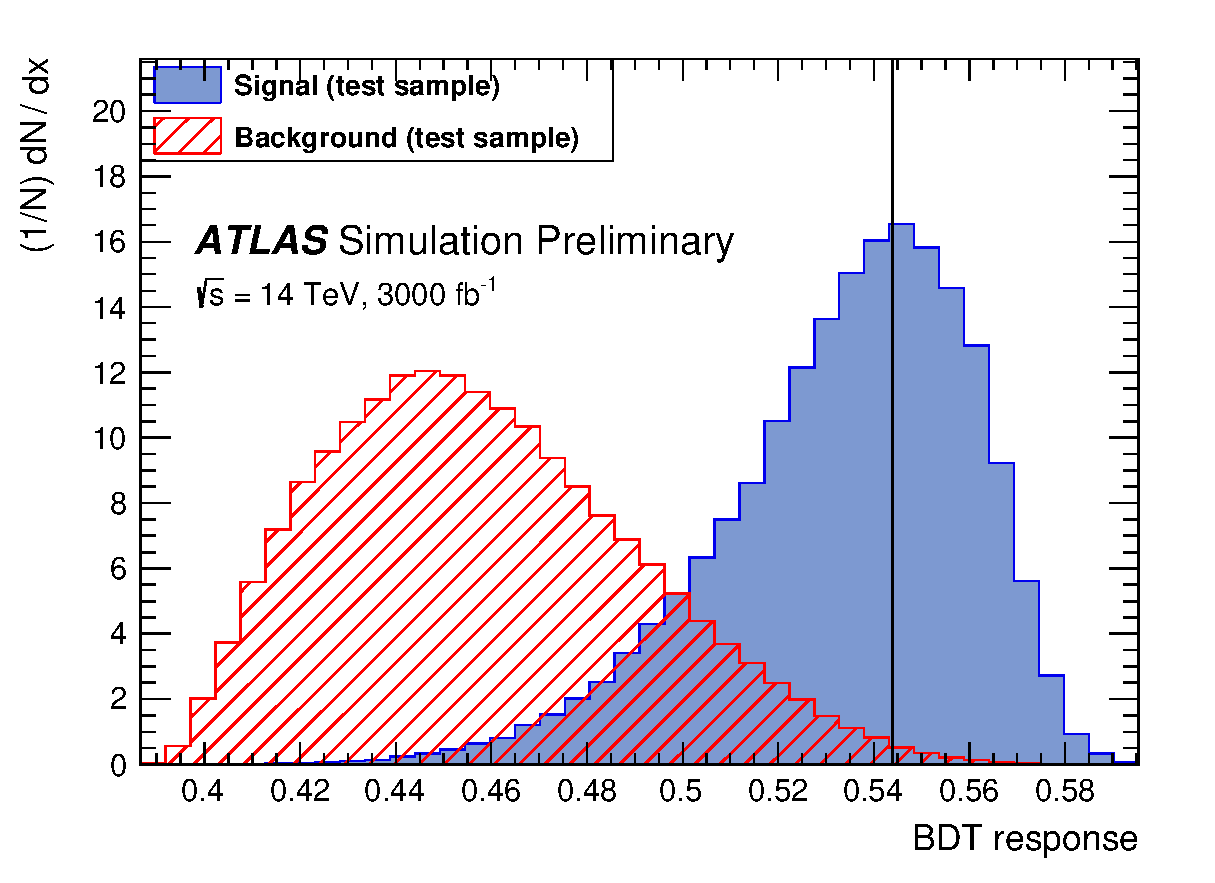
\includegraphics[width=0.5\textwidth]{Ch6/Img/figures_bbyy_overtrainTestOnly.eps}
    \caption{BDT response for signal and background. The vertical line denotes the optimal cut on the BDT response that maximises the statistical-only significance,}
    \label{fig:HL-LHC:36ifb:BDT}
\end{figure}

A BDT cut is set at 0.54 to define a single category that maximizes the statistical-only significance. The BDT selects around 40\% of the SM HH signal, while it rejects almost 99\% of backgrounds. The analysis used the $m_{\gamma\gamma\bar{b}b}$ shape fit in the \myy $\in$[123, 127] GeV window to extract the results. The sensitivity to \kl is enhanced by defining 8 bins in the $m_{\gamma\gamma\bar{b}b}$ distribution. The negative log-likelihood ratio performed on an Asimov data set generated with \kl=1 is shown in Figure \ref{fig:HL-LHC:36ifb:LH}. Table \ref{tab:HL-LHC:36ifb:kl} summarized constraints on \kl from the likelihood ratio test. It shows that even with 3000 \ifb the analysis still statistically dominated.
\begin{figure}[htbp]
    \centering
    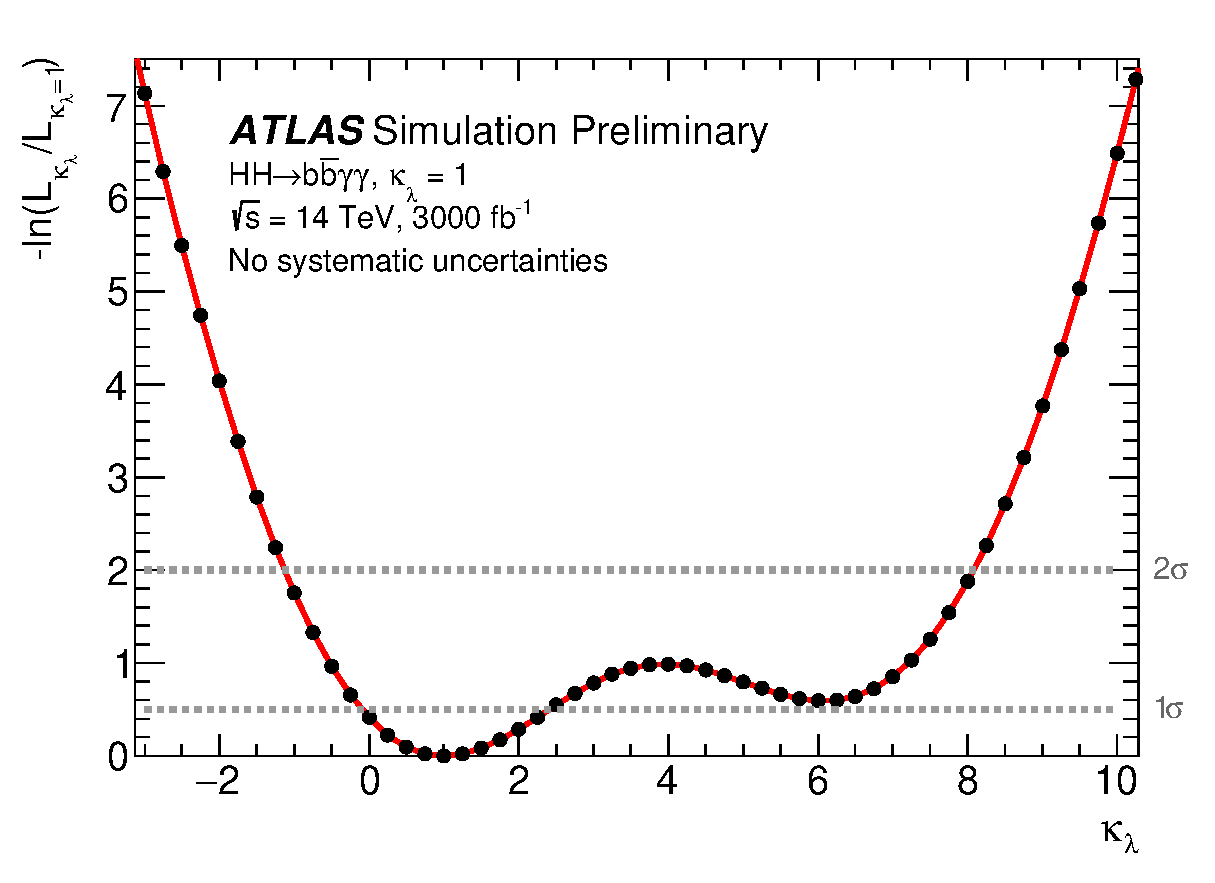
\includegraphics[width=0.5\textwidth]{Ch6/Img/figures_bbyy_NoSyst_likelihoodCurve_-3to10.eps}
    \caption{Negative natural logarithm of the ratio of the maximum likelihood for \kl to the maximum likelihood for \kl = 1 for the fit with only statistical uncertainties.}
    \label{fig:HL-LHC:36ifb:LH}
\end{figure}

\begin{table}[htbp]
    \centering
    \begin{tabular}{lcc}
\hline \hline Scenario & $1 \sigma \mathrm{CI}$ & $2 \sigma \mathrm{CI}$ \\
\hline No systematic uncertainties & $-0.1<\kappa_{\lambda}<2.4$ & $-1.1<\kappa_{\lambda}<8.1$ \\
Systematic uncertainties included & $-0.2<\kappa_{\lambda}<2.5$ & $-1.4<\kappa_{\lambda}<8.2$ \\
\hline \hline
\end{tabular}
    \caption{Constraints on \kl from the likelihood ratio test performed on the Asimov dataset created from the backgrounds and the SM HH signal.}
    \label{tab:HL-LHC:36ifb:kl}
\end{table}

\subsection{Combination with \bbbb and \bbtt channels}

An extrapolation of the 36 \ifb analysis of \bbbb and \bbtt channels to HL-LHC was also performed (More details in Reference ). Their statistical combination is performed by constructing a combined likelihood function that takes into account Asimov, signal and background models and correlated systematic uncertainties from all channels as well as orthogonality between channels. Figure \ref{fig:HL-LHC:Comb:LH} shows the combined likelihood scan. The combined significance for SM HH is evaluated to be 3.5$\sigma$ without systematic uncertainties and 3$\sigma$ including systematic and its mainly driven by \bbtt and \bbyy channels as shown in Figure \ref{fig:HL-LHC:Comb:sig}. The significance depends on the expected signal yield and therefore it is lower for those \kl values for which the cross-section and the acceptance times efficiency is low. The measured combined signal strength is 1.0 $\pm$ 0.4 including systematic and 1.0 $\pm$ 0.3 without systematic. Tables \ref{tab:HL-LHC:Comb:sig} and \ref{tab:tab:HL-LHC:Comb:mu} show the significance and the signal strength measured in the individual HH channels, respectively. 


Table \ref{tab:HL-LHC:Comb:CI} resumes the constraints on \kl from the likelihood test performed on the Asimov dataset created from the backgrounds and HH signal with \kl= 1.  


\begin{figure}[htbp]
    \centering
    \includegraphics[width=0.5\textwidth]{Ch6/Img/figures_combination_bbbb_bbtt_bbyy_lHHH0100_NoSyst_overlay_Preliminary.pdf}
    \caption{Negative natural logarithm of the ratio of the maximum likelihood for \kl to the maximum likelihood for \kl = 1 for the fit with only statistical uncertainties. The black circles show the results for the combination, while the coloured markers show the values coming from the individual channels.}
    \label{fig:HL-LHC:Comb:LH}
\end{figure}

\begin{figure}[htbp]
    \centering
    \includegraphics[width=0.5\textwidth]{Ch6/Img/figures_combination_bbbb_bbtt_bbyy_NoSyst_Significance_Preliminary.pdf}
    \caption{Expected significance of observing Higgs-boson-pair production as a function of \kl without any systematic uncertainties.  The two horizontal dashed lines show the 3$\sigma$ and 5$\sigma$ thresholds.} 
    \label{fig:HL-LHC:Comb:sig}
\end{figure}

\begin{table}[htbp]
    \centering
    \begin{tabular}{lcc}
\hline \hline
Channel & Statistical-only & Statistical + Systematic \\
\hline
$H H \rightarrow b \bar{b} b \bar{b}$ & $1.4$ & $0.61$ \\
$H H \rightarrow b \bar{b} \tau^{+} \tau^{-}$ & $2.5$ & $2.1$ \\
$H H \rightarrow b \bar{b} \gamma \gamma$ & $2.1$ & $2.0$ \\
\hline Combined & $3.5$ & $3.0$ \\
\hline \hline
\end{tabular}
    \caption{Significance of the individual \bbbb, \bbtt and \bbyy channels as well as their combination.}
    \label{tab:HL-LHC:Comb:sig}
\end{table}

\begin{table}[htbp]
    \centering
    \begin{tabular}{lcc}
\hline \hline 
Channel & Measured $\mu$ (Statistical-only) & Measured $\mu$ (Statistical + Systematic) \\
\hline
$H H \rightarrow b \bar{b} b \bar{b}$ & $1.0 \pm 0.6$ & $1.0 \pm 1.6$ \\
$H H \rightarrow b \bar{b} \tau^{+} \tau^{-}$ & $1.0 \pm 0.4$ & $1.0 \pm 0.5$ \\
$H H \rightarrow b \bar{b} \gamma \gamma$ & $1.0 \pm 0.6$ & $1.0 \pm 0.6$ \\
\hline Combined & $1.00 \pm 0.31$ & $1.0 \pm 0.4$ \\
\hline \hline
\end{tabular}
    \caption{Signal strength measured in the individual channels and their combination using an Asimov dataset with SM HH signal injected.}
    \label{tab:tab:HL-LHC:Comb:mu}
\end{table}

\begin{table}[htbp]
    \centering
    \begin{tabular}{lcc}
\hline \hline Scenario & $1 \sigma \mathrm{CI}$ & $2 \sigma \mathrm{CI}$ \\
\hline Statistical uncertainties only & $0.4 \leq \kappa_{\lambda} \leq 1.7$ & $-0.10 \leq \kappa_{\lambda} \leq 2.7 \cup 5.5 \leq \kappa_{\lambda} \leq 6.9$ \\
Systematic uncertainties & $0.25 \leq \kappa_{\lambda} \leq 1.9$ & $-0.4 \leq \kappa_{\lambda} \leq 7.3$ \\
\hline \hline
\end{tabular}
    \caption{Constraints on \kl from the likelihood ratio test performed on the Asimov dataset created from the backgrounds and the SM HH signal. Results are presented as 1$\sigma$ and 2$\sigma$ CI on \kl.}
    \label{tab:HL-LHC:Comb:CI}
\end{table}






\subsection{Extrapolation of full Run-2 analysis}

To test the performance of the full Run-2 analysis at HL-LHC, an extrapolation to 3000 \ifb is performed. The extrapolation is performed under the assumption that the planned upgrades to the ATLAS detector and improvements to reconstruction algorithms will mitigate the effects of higher pile-up, resulting in the same Run-2 detector performances. For simplicity, the 139 \ifb analysis strategy is kept unchanged and a simple luminosity scaling is performed. No systematic uncertainties are considered since the European strategy study shows that \bbyy analysis still statistically dominated even at HL-LHC. The effect of energy increase on the cross-section is neglected. An increase of the analysis sensitivity is expected from further analysis strategy optimization, while the global developments of the analysis are hard to predict over many years of R\&D. The extrapolation aims at giving a realistic estimation of the expected sensitivity gain using the current state-of-the-art analysis methods. \\

An Asimov dataset with the background-only hypothesis was created, and maximum likelihood fits of this dataset were performed with different \kl hypotheses. The negative logarithm of the ratio of the maximum likelihood for \kl to that for the fit with \kl= 1 is shown in Figure \ref{fig:HL-LHC:LH}. The 1$\sigma$ and the 2$\sigma$ confidence interval (CI) constraints on \kl from the full Run-2 analysis, the European strategy and the extrapolation of the full Run-2 analysis to HL-LHC are shown in Table \ref{tab:HL-LHC:kl}. 

\begin{figure}[htbp]
    \centering
    \includegraphics[width=0.5\textwidth]{Ch6/Img/likelihood_subplot.pdf}
    \begin{tcolorbox}[colback=black!5!white, colframe=white!75!black]
    \caption{Negative natural logarithm of the ratio of the maximum likelihood for \kl to the maximum likelihood for \kl= 1. The dashed lines at 0.5 and 2.0 indicate the values corresponding to a 1$\sigma$ and 2$\sigma$ confidence interval, respectively (assuming an asymptotic $\chi^2$ distribution of the test statistic).}
    \label{fig:HL-LHC:LH}
    \end{tcolorbox}
\end{figure}

\begin{table}[htbp]
    \centering
    \begin{tabular}{lcc}
    \hline\hline 
        Scenario & 1$\sigma$ CI & 2$\sigma$ CI \\
    \hline    
        Run-2 Stat. Only & [-1.3, 6.4]  & [-2.9, 8] \\ 
        European Strategy Stat. Only & [-0.1, 2.4] & [-1.1, 8.1] \\
        Extrapolation to HL-LHC Stat. Only & [0.4, 1.9] & [-0.1, 4.7] \\
    \hline\hline 
    \end{tabular}
    \begin{tcolorbox}[colback=black!5!white, colframe=white!75!black]
    \caption{Constraints on \kl from the likelihood ratio rest performed on the Asimov dataset created from the background and the \kl= 1 signal, as shown in Figure \ref{fig:HL-LHC:LH}.}
    \label{tab:HL-LHC:kl}
    \end{tcolorbox}
\end{table}

The expected median significance of the SM HH signal relative to the background-only hypothesis for individual category and their combination is shown in Table \ref{tab:HL-LHC:Sig} and the measured signal strength 1.0 $\pm$ 0.28. A factor 2 improvement in the signal strength accuracy is achieved. 

\begin{table}[htbp]
    \centering
    \begin{tabular}{lcc}
    \hline\hline 
        Scenario & Run-2 Stat. Only & HL-LHC Stat. Only \\
    \hline    
        High mass, High BDT & 0.47 & 2.17 \\
        High mass, Low BDT  & 0.13 & 0.58 \\
        Low mass, High BDT  & 0.03 & 0.14 \\
        Low mass, Low BDT   & 0.02 & 0.09 \\
        \hline
        Combined & 0.48$\sigma$ & 2.25$\sigma$ \\
    \hline\hline 
    \end{tabular}
    \begin{tcolorbox}[colback=black!5!white, colframe=white!75!black]
    \caption{The Statistical-only significance of the individual categories as well as their combination.}
    \label{tab:HL-LHC:Sig}
    \end{tcolorbox}
\end{table}

The HL-LHC extrapolation of the Run-2 analysis shows similar performance for the SM HH to the European strategy results while it shows a better \kl constraint. This is mainly driven by the BDT strategy used. As mentioned before, the European strategy study uses a single BDT trained on SM HH and define a single signal region. By construction, this signal region is equivalent to the High mass, High BDT category defined for full Run-2 analysis from which the significance is mostly driven. This explains the similarity in analysis performance. For \kl sensitivity, having a dedicated BDT targeting (Low mass) trained on \kl = 10 HH signal, mostly improves the full Run-2 sensitivity for \kl variations. This explains the improved \kl constraint. Figure shows the significance as a function of \kl from the extrapolation of full Run-2 analysis and the European strategy results. \\

\section{Conclusion}

A prospect study for the search for non-resonant Higgs-boson-pair production at the HL-LHC has been performed, using the \bbbb, \bbyy and \bbtt channels and their combination. From the European strategy combination, the signal strength is expected to be measured with an accuracy of 30\% and the \kl is constrained at 95\% to [-0.1, 2.7] $\cup$ [5.5, 6.9]. The full Run-2 \HHyybb analysis presented in this thesis is statistically extrapolated to HL-LHC. From 139 \ifb \HHyybb extrapolation, the signal strength is expected to be measured with an accuracy of 28\% and the Higgs self-coupling is constrained at 95\% to [-0.1, 4.7]. Improving the sensitivity of the \HHyybb in the future through enhancement of \mbb, analysis strategy and photon identification is possible.  
